%!TEX root = ../thesis.tex

\section{背景}
AIFormulaは計測自動制御学会と自動車技術会が主催し, 本田技術研究所がサポートする次世代の人工知能モビリティの競技会で, 正式な競技会は2025年から始まる.
\cite{aiformula}
AIFormulaは今後ますます需要が高まるであろう自動化システムの技術者を育てるという点で効果が見込まれる.
AIFormulaではハードウェアの変更もある程度許容されているが, 現時点での開発はソフトウェアが中心となる.
ハードウェアは経路追従するために必要なパーツが全て揃っているが, ソフトウェアはデバイスを駆動するサンプルプログラムが用意されているのみである.
\cite{aiformula-support}
競技という性質上, 経路追従などのソフトウェアは各チームで開発することが必要となる.
\cite{aiformula-chibakou}
\cite{aiformula-repo}
その点で, コースを自動で走行するためにはソフトウェアの開発は必須となる.

\subsection{ハードウェア}
AIFormulaでは詳細なルールは検討中であるとのことで, 2025年2月に開催される予定のプレ大会以降に詳細なルールが決定される予定となっている.
Fig.1.1に2025年のプレ大会で使用される予定のロボットを示す.
ロボットは本田技術研究所から貸与されたロボットを使用していて, 差動二輪と一輪のキャスタ(以下, 従動輪と呼ぶ)で構成された三輪モデルである.
バッテリーにはMPP(Mobile Power Pack)が使用される. MPPは持ち運び可能な交換式バッテリーとなっている. Fig.1.2にMPPを示す.
プレ大会では指定されたコースを3周する時間で競われる.

\begin{figure}[H]
  \centering
 \includegraphics[keepaspectratio, scale=0.6]
      {images/ExteriorViewOfTheMobilityPlatform.png}
 \caption{Exterior view of the mobility platform}
 \label{fig:robot view}
\end{figure}

\begin{figure}[H]
  \centering
 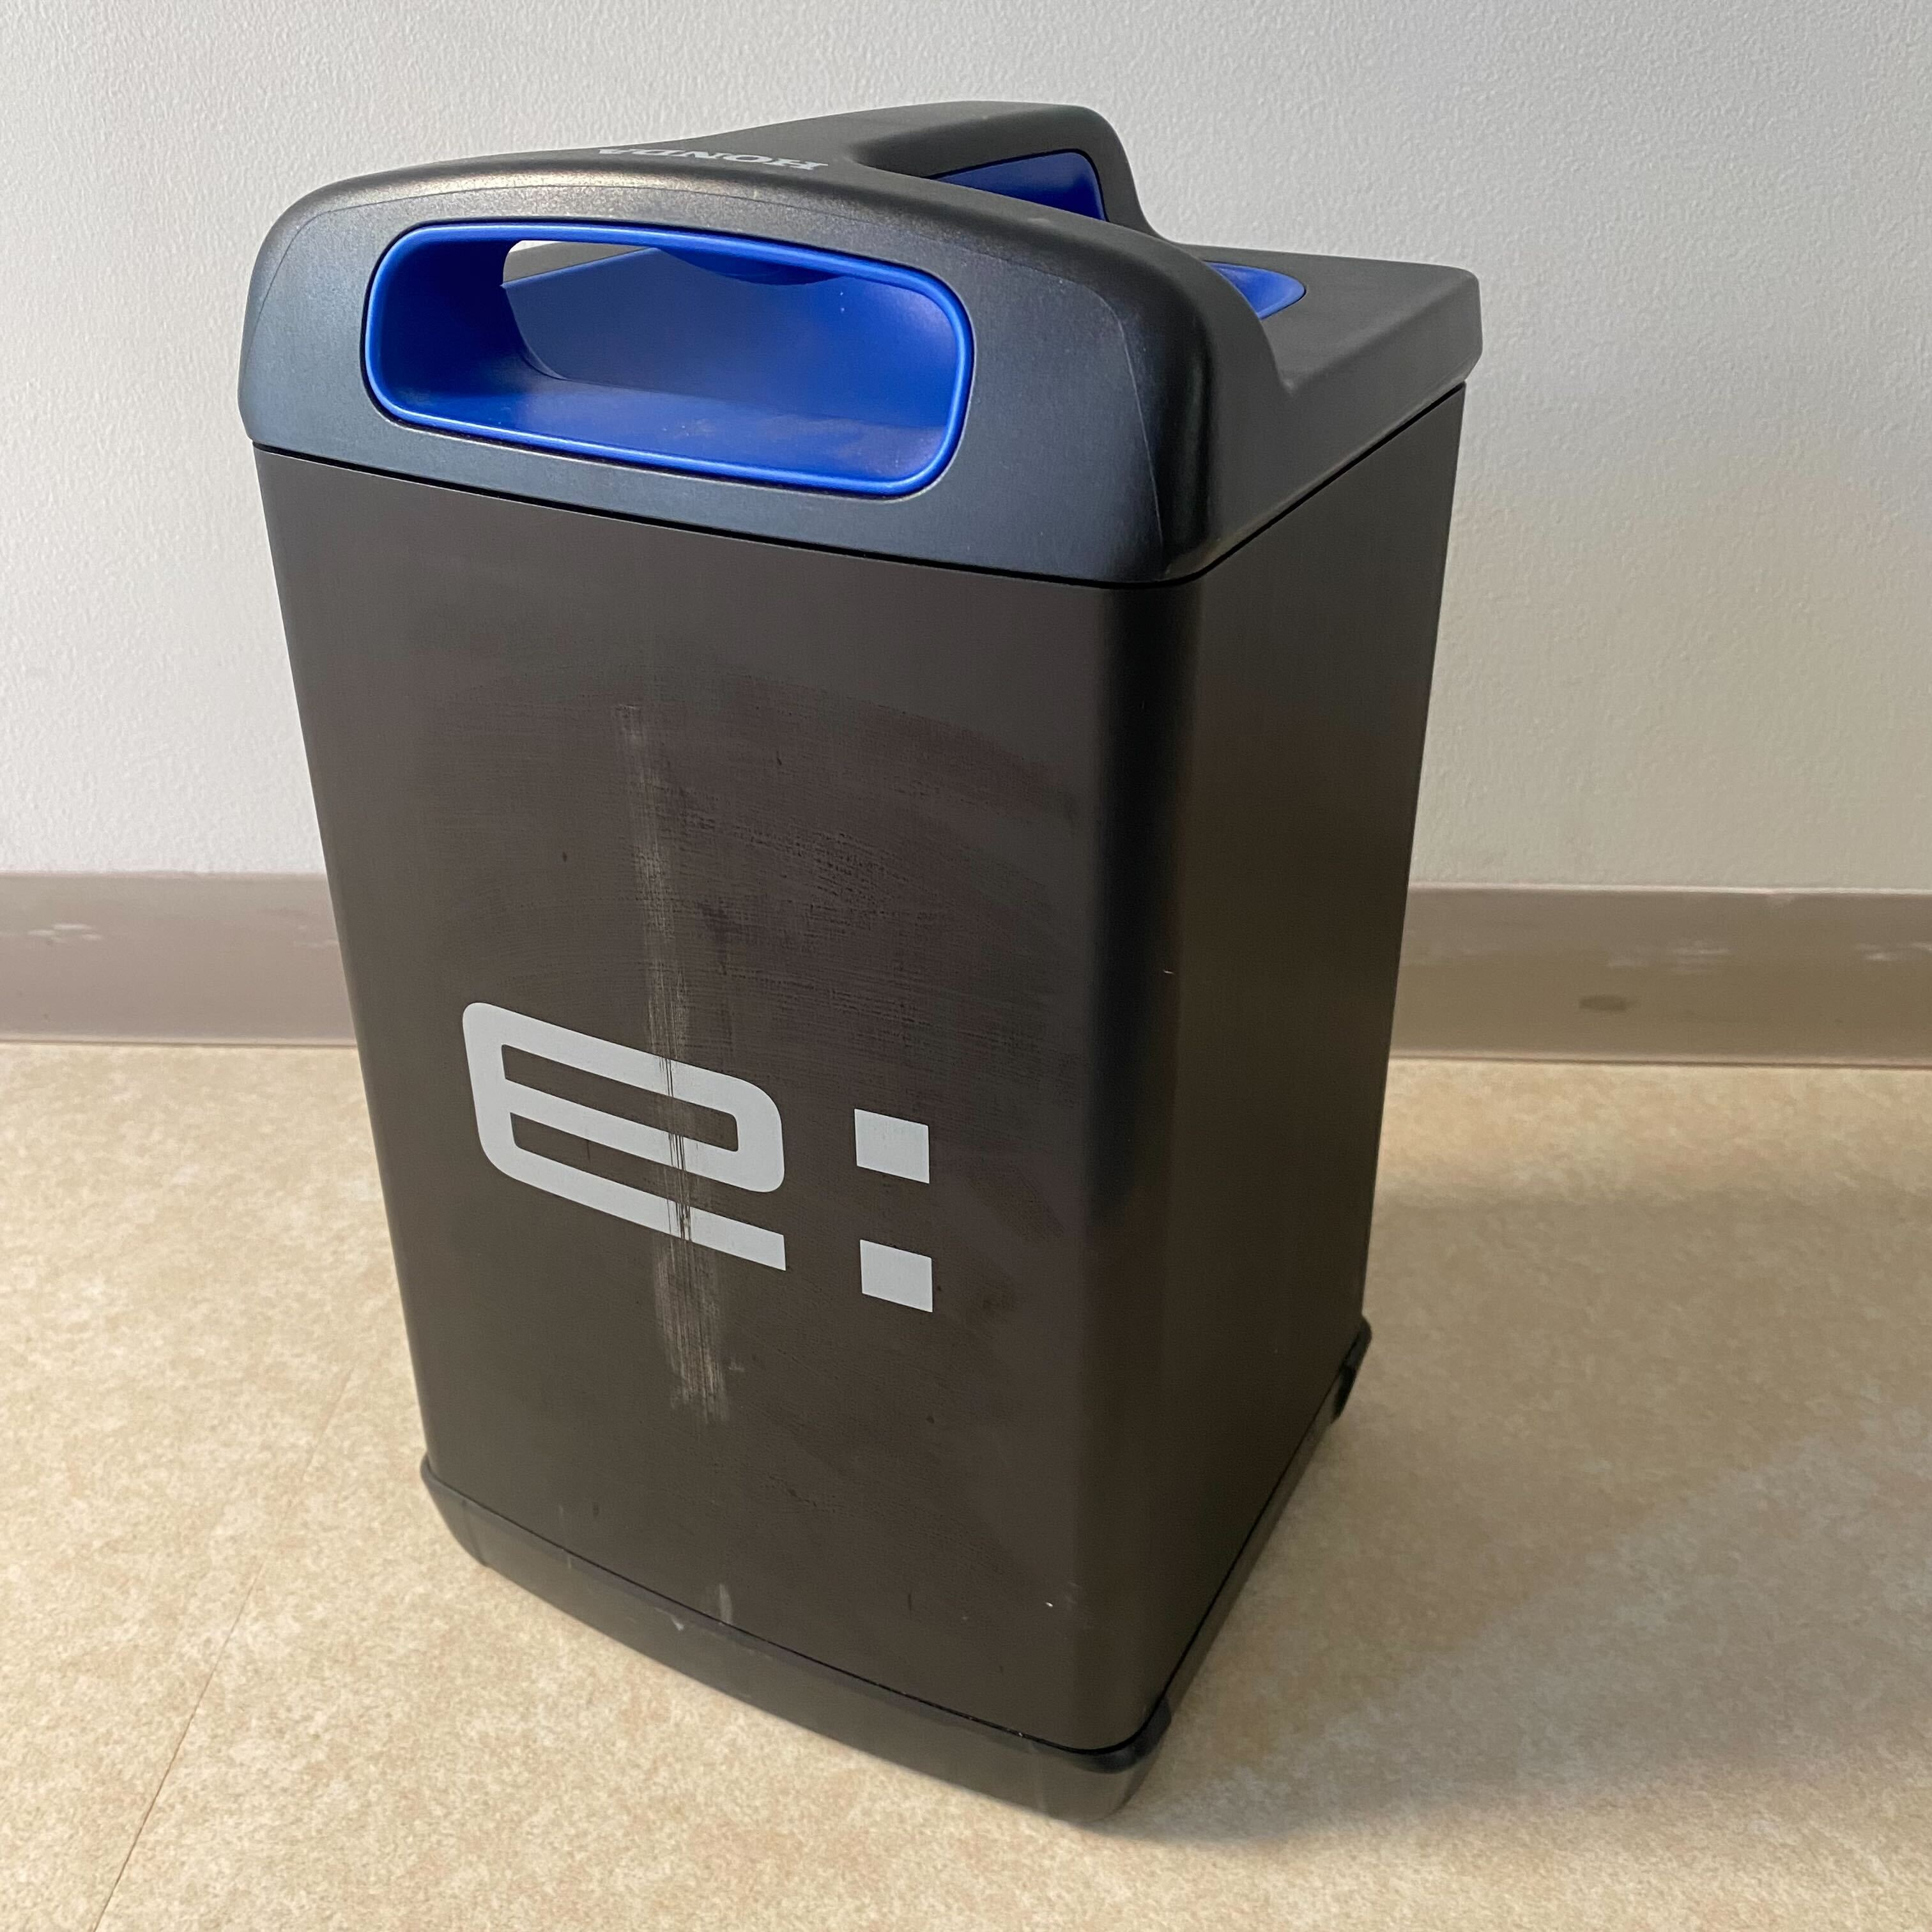
\includegraphics[keepaspectratio, scale=0.08]
      {images/mpp.png}
 \caption{Mobile Power Pack}
 \label{fig:MPP}
\end{figure}

\subsection{レギュレーション}
詳細なルールは検討中の段階であるが, Table.1.1に現時点で判明しているレギュレーションについて示す.

\begin{table}[H]
     \centering
     \caption{regulation}
     \begin{tabular}{|c|c|lll}
     \cline{1-2}
                              & レギュレーション              &  &  &  \\ \cline{1-2}
                                   & 車体寸法, モータ, バッテリー(MPP), タイヤは統一 &  &  &  \\
     ハードウェア                       & 三輪モデル(差動二輪+従動輪)               &  &  &  \\
                                   & LiDAR使用禁止                     &  &  &  \\
                                   & 一部基板ソフトウェア変更不可                &  &  &  \\ \cline{1-2}
     \multicolumn{1}{|l|}{ソフトウェア} & 高精度地図の使用禁止                    &  &  &  \\
     \multicolumn{1}{|l|}{}       & Autowareパッケージの使用禁止            &  &  &  \\ \cline{1-2}
     \end{tabular}
\end{table}

\subsection{コース}
Fig.1.3にAIFormulaのコースを示す.
周囲に高い建造物のない平坦なコースである.


\begin{figure}[H]
  \centering
 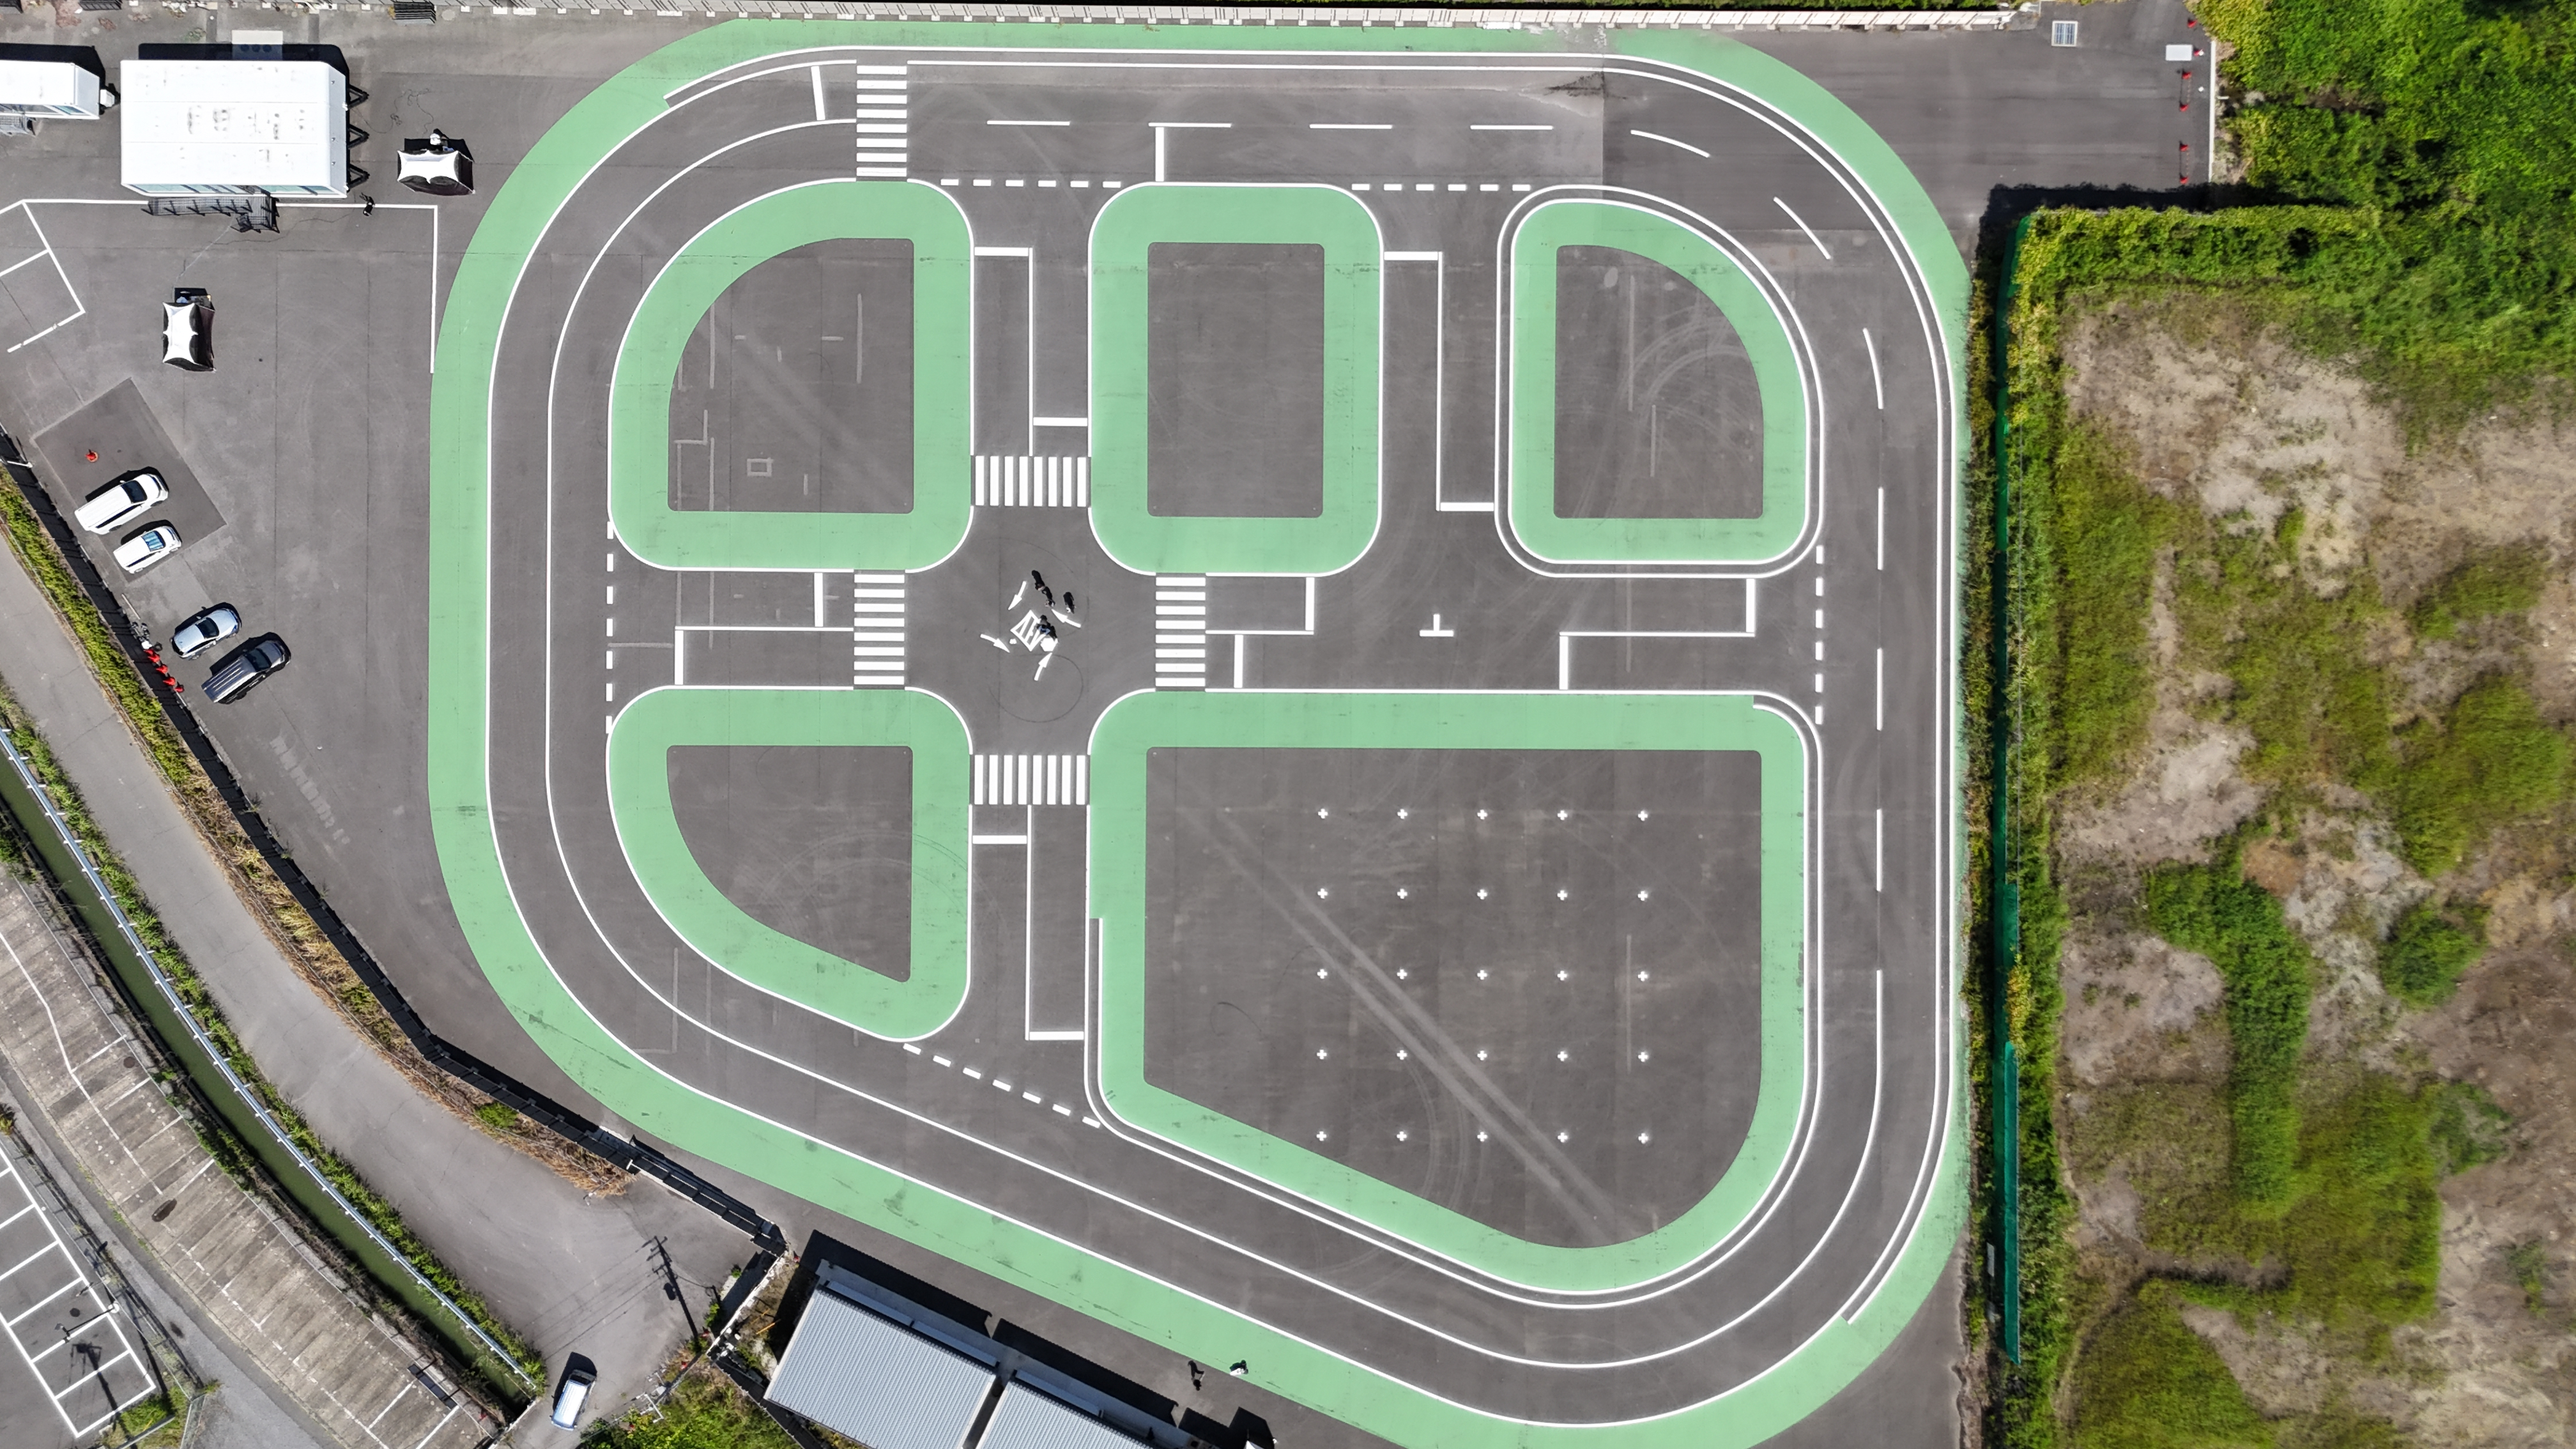
\includegraphics[keepaspectratio, scale=0.1]
      {images/AerialViewAndMobilitysPerspetiveOfTheCourse.png}
 \caption{Aerial view and mobility perspective of the course}
 \label{fig:course}
\end{figure}


\section{目的}
本研究では, 経路追従をするパッケージを開発して評価を行うことで作成した経路追従ソフトウェアの有効性を実環境で検証することを目的とする.


\section{論文の構成}
本論文は以下のように構成される.
まず, 2章で本研究で使用される要素技術について述べる.
3章では経路追従する際に使用するアルゴリズムについて述べる.
4章では開発した経路追従ソフトウェアに要求されるシステムについてまとめる.
5章ではシミュレータ環境で経路追従の実験を行い, アルゴリズムの有効性を確認する.
6章では実環境で経路追従の実験を行う.
7章では本研究の結論をまとめる.

\newpage
